\section{Расположения прямой и окружности}

\paragraph{Точки внутри круга и точки вне его.}\label{1914/118}
Окружность разделяет все точки плоскости на три области:

\begin{wrapfigure}{r}{33mm}
\centering
\includegraphics{mppics/ris-1914-113}
\caption{}\label{1914/ris-113}
\bigskip
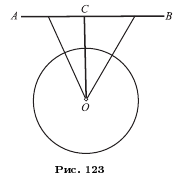
\includegraphics{mppics/ris-123}
\caption{}\label{1938/ris-123}
\bigskip
\includegraphics{mppics/ris-124}
\caption{}\label{1938/ris-124}
\bigskip
\includegraphics{mppics/ris-125}
\caption{}\label{1938/ris-125}
\end{wrapfigure}


1) точки \rindex{внешние точки круга}\textbf{вне круга}, расстояние от которых до центра больше радиуса; 

2) точки на окружности, расстояние от которых до центра равны радиусу; 

3) точки \rindex{внутренние точки круга}\textbf{внутри круга}, расстояние от которых до центра меньше радиуса. 

Следующее утверждение мы принимаем за очевидное:

\emph{Если отрезок (или дуга) соединяет точку \emph{($A$ рис.~\ref{1914/ris-113})} внутри круга с какою-нибудь точкой \emph{($B$)} вне его, то он пересекается где-нибудь с окружностью \emph{(в точке $X$ для отрезка $AB$ и в точках $Y$ и $Z$ для двух дуг с концами в $A$ и $B$)}.}

%%%добавлено допущения о пересечениях 119(1914)

\paragraph{}\label{1938/112}
Прямая и окружность могут, очевидно, находиться только в следующих трёх относительных положениях.


1) \emph{Расстояние \emph{($OC$)} от центра до прямой \emph{($AB$) (то есть длина перпендикуляра $OC$, опущенного из центра на прямую)} больше радиуса окружности} (рис.~\ref{1938/ris-123}).
Тогда точка $C$ прямой удалена от центра больше, чем на радиус, и потому лежит вне круга.
Так как все остальные точки прямой удалены от $O$ ещё более, чем точка $C$ (наклонные длиннее перпендикуляра), то они все лежат вне круга;
значит, тогда прямая не имеет никаких точек, общих с окружностью.

2) \emph{Расстояние \emph{($OC$)} от центра до прямой меньше радиуса.}
В этом случае (рис.~\ref{1938/ris-124}) точка $C$ лежит внутри круга. 
Но на прямой $AB$, по обе стороны от точки $C$, можно найти такие точки $D$ и $E$, которые удалены от $O$ более, чем на радиус%
\footnote{Если, например, на прямой $AB$ отложим от точки $C$ по обе стороны от неё, отрезки, большие радиуса, то расстояние их концов до центра будут больше радиуса, так как перпендикуляр короче наклонной.}
и которые, следовательно, лежат вне круга.
Но тогда каждый из двух отрезков: $CD$ и $CE$, соединяя внутреннюю точку с внешней, должен пересечься с окружностью (§~\ref{1914/118}).
Следовательно, в этом случае прямая имеет с окружностью 2 общие точки.
%вернул доказательство из 1914/135

3) \emph{Расстояние \emph{($OC$)} центра от прямой равно радиусу.}
Тогда точка $C$ (рис.~\ref{1938/ris-125}) принадлежит и прямой и окружности, все же остальные точки прямой, будучи удалены от $O$ более, чем точка $C$, лежат вне круга.
Значит, в этом случае прямая и окружность имеют только одну общую точку, именно ту, которая служит основанием перпендикуляра, опущенного из центра на прямую.

Такая прямая, которая с окружностью имеет только одну общую точку, называется \rindex{касательная}\textbf{касательной} к окружности;
общая точка называется \rindex{точка!касания}\textbf{точкой касания}.

\begin{wrapfigure}{o}{45mm}
\centering
\includegraphics{mppics/ris-1914-134}
\caption{}\label{1914/ris-134}
\end{wrapfigure}

\medskip

\smallskip
\mbox{\so{Замечание}.}
Когда речь идёт о произвольной гладкой кривой, то за определение касательной принимают \emph{предельное положение} $MT$, к которому стремится секущая $MP$, когда точка $P$ скользит по кривой неограниченно приближаясь к $M$.
Для окружности оба определения равносильны, но в общем случае, определяемая таким образом касательная может иметь с кривой более одной общей точки (рис.~\ref{1914/ris-134}).% из 143(1914)

\paragraph{}\label{1938/113}
Относительно касательной мы докажем следующие \so{две теоремы} (прямую и обратную):

1) \textbf{\emph{если прямая}} ($MN$ рис.~\ref{1938/ris-126}) \textbf{\emph{перпендикулярна к радиусу}} ($OA$) \textbf{\emph{в конце его}} ($A$), \textbf{\emph{лежащем на окружности, то она касается окружности,}} и обратно,

2) \textbf{\emph{если прямая касается окружности, то радиус, проведённый в точку касания, перпендикулярен к ней.}}

\begin{wrapfigure}{o}{33mm}
\centering
\includegraphics{mppics/ris-126}
\caption{}\label{1938/ris-126}
\end{wrapfigure}

1) Точка $A$, как конец радиуса, лежащий на окружности, принадлежит этой окружности;
в то же время она принадлежит и прямой $MN$.
Значит, эта точка есть общая у окружности и прямой.
Все же остальные точки прямой $MN$, как $B$, $C$ и другие, отстоят от центра $O$ дальше, чем на радиус (так как отрезки $OB$, $OC,\dots$, как наклонные, больше перпендикуляра $OA$), и потому они лежат вне окружности.
Таким образом, у прямой $MN$ есть только одна точка ($A$), общая с окружностью, и, значит, прямая $MN$ есть касательная.

2) Пусть $MN$ касается окружности в точке $A$; требуется доказать, что $MN\perp OA$.
Предположим противное, то есть что радиус $OA$ не перпендикулярен к $MN$, а представляет собою наклонную к этой прямой.
В таком случае какая-нибудь другая прямая, например $OC$, будет перпендикуляром, опущенным из центра $O$ на касательную $MN$ (§~\ref{1938/24}).
Значит найдётся другая точка $A'$ на $MN$ лежащая от $C$ на том же расстоянии, что и $A$.
В этом случае, $OA=OA'$ (§~\ref{1938/54});
то есть $MN$ имеет две общие точки с окружностью и значит не может её касаться.
% почти возвратщено к версии 1914

\begin{wrapfigure}{r}{33mm}
\centering
\includegraphics{mppics/ris-1931-149}
\caption{}\label{1931/ris-149}
\bigskip
\includegraphics{mppics/ris-127}
\caption{}\label{1938/ris-127}
\bigskip
\includegraphics{mppics/ris-128}
\caption{}\label{1938/ris-128}
\end{wrapfigure}

\smallskip
\mbox{\so{Следствие}.}
\emph{Две касательные, проведённые к окружности из точки вне её, равны и образуют равные углы с прямой, соединяющей эту точку с центром,} что следует из равенства прямоугольных треугольников $AOB$ и $AOB_1$ (рис.~\ref{1931/ris-149}).

\paragraph{}\label{1938/114}
\mbox{\so{Теорема}.}
\textbf{\emph{Если касательная параллельна хорде, то точка касания делит дугу, стягиваемую хордой, пополам.}}

Пусть прямая $AB$ касается окружности в точке $M$ (рис.~\ref{1938/ris-127}) и параллельна хорде $CD$;
требуется доказать, что ${\smallsmile}CM={\smallsmile}MD$.

Проведя через точку касания диаметр $ME$, будем иметь:
$EM\perp AB$ и, следовательно, $EM\z\perp CD$;
поэтому ${\smallsmile}CM\z={\smallsmile}MD$.

\paragraph{}\label{1938/115}
\mbox{\so{Задача}.}
\emph{Провести касательную к данной окружности с центром $O$ параллельно данной прямой $AB$} (рис. \ref{1938/ris-128}).

Опускаем на $AB$ из центра $O$ перпендикуляр $OC$ и через точку $D$, в которой этот перпендикуляр пересекается с окружностью, проводим $EF\parallel AB$.
Искомая касательная будет $EF$.
Действительно, так как $OC\perp AB$ и $EF\parallel AB$, то $EF\perp OD$, а прямая, перпендикулярная к радиусу в конце его, лежащем на окружности, есть касательная.


\paragraph{}\label{1931/115}
\mbox{\so{Задача}.}
\emph{Через данную точку провести касательную к данной окружности.}
Если данная точка (например, точка $C$, рис. \ref{1938/ris-125}) находится на окружности, то проводят через неё радиус и через конец радиуса перпендикулярную прямую.
Эта прямая и будет искомой касательной.
Другой касательной через ту же точку окружности провести нельзя, так как касательная должна быть перпендикулярна к радиусу в конце его, лежащем на окружности, а двух различных перпендикуляров к одному и тому же радиусу через одну и ту же точку провести нельзя.

Рассмотрим случай, когда точка дана вне круга.
Пусть требуется (рис. \ref{1931/ris-124}) провести к окружности с центром $O$ касательную через точку $A$.
Для этого из точки $A$ как из центра описываем дугу радиуса $AO$, а из точки $O$ как из центра пересекаем эту дугу в точках $B$ и $C$ раствором циркуля, равным удвоенному радиусу данной окружности.
Проведя затем хорды $OB$ и $OC$, соединим точку $A$ с точкам и $D$ и $E$, в которых эти хорды пересекаются с
данной окружностью.
Прямые $AD$ и $AE$ и будут касательными к данной окружности.

\begin{wrapfigure}{o}{32mm}
\centering
\includegraphics{mppics/ris-1931-124}
\caption{}\label{1931/ris-124}
\end{wrapfigure}

Действительно, из построения видно, что $\triangle AOB$ и $\triangle AOC$ равнобедренные ($AO=AB\z=AC$) с основаниями $OB$ и $OC$, равными удвоенному радиусу окружности.
Так как $OD$ и $OE$ — радиусы, то $D$ есть середина $OB$, а $E$ — середина $OC$.
Значит, прямые $AD$ и $AE$ являются медианами, проведёнными к основаниям равнобедренных треугольников и потому перпендикулярны к этим основаниям (§~\ref{1938/38}).
Если же прямые $AD$ и $AE$ перпендикулярны к радиусам $OD$ и $OE$ в их концах, лежащих
на окружности, то они касательные (§~\ref{1938/113}).

\smallskip
\so{Замечание}. Ниже (§~\ref{1938/128}) будет указан другой приём проведения касательной.

{

\begin{wrapfigure}{r}{48mm}
\vskip-3mm
\centering
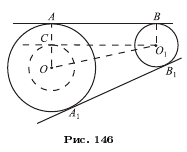
\includegraphics{mppics/ris-146}
\caption{}\label{1938/ris-146}
\end{wrapfigure}

\paragraph{}\label{1938/129}
\mbox{\so{Задача}.}
\emph{К двум окружностям с центрами $O$ и $O_1$ провести общую касательную} (рис.~\ref{1938/ris-146}).

1) \so{Анализ}.
Предположим, что задача решена.
Пусть $AB$ будет общая касательная, $A$ и $B$ — точки касания.
Очевидно, что если мы найдём одну из этих точек, например $A$, то затем легко найдём и другую.
Проведём радиусы $OA$ и $O_1B$.
Эти радиусы, будучи перпендикулярны к общей касательной, параллельны между собой;
поэтому, если из $O_1$ проведём $O_1C\parallel BA$, то треугольник $OCO_1$ будет прямоугольный с прямым углом при вершине $C$;
вследствие этого, если опишем с центром в точке $O$ радиусом $OC$ окружность, то она будет касаться прямой $O_1C$ в точке $C$.
Радиус этой вспомогательной окружности известен:
он равен $OA-CA=OA-O_1B$, то есть
он равен разности радиусов данных окружностей.

}

\smallskip
\so{Построение}.
Таким образом, построение можно выполнить так:
описываем окружность с центром в точке $O$ радиусом, равным разности данных радиусов;
из $O_1$ проводим к этой окружности касательную $O_1C$ (способом, указанным в предыдущей задаче);
через точку касания $C$ проводим радиус $OC$ и продолжаем его до встречи с данной окружностью в точке $A$.
Наконец, из $A$ проводим $AB$ параллельно $CO_1$.

Совершенно таким же способом мы можем построить другую общую касательную $A_1B_1$.
Прямые $AB$ и $A_1B_1$ называются \rindex{внешние касательные}\textbf{внешними касательными} двух окружностей.

Аналогично можно построить и \rindex{внутренние касательные}\textbf{внутренние касательные} (рис. \ref{1938/ris-147}).

\begin{wrapfigure}{o}{48mm}
\centering
\includegraphics{mppics/ris-147}
\caption{}\label{1938/ris-147}
\end{wrapfigure}

2) \so{Анализ}.
Предположим, что задача решена.
Пусть $AB$ будет искомая касательная.
Проведём радиусы $OA$ и $O_1B$ в точки касания $A$ и $B$.
Эти радиусы, будучи оба перпендикулярны к общей касательной, параллельны между собой.

Поэтому, если из $O_1$ проведём $O_1C\parallel BA$ и продолжим $OA$ до пересечения с $O_1C$ в точке $C$, то $OC$ будет перпендикулярен к $O_1C$, вследствие этого окружность, описанная радиусом $OC$ с центром в точке $O$, будет касаться прямой $O_1C$ в точке $C$.
Радиус этой вспомогательной окружности известен, он равен:
$OA+AC=OA+O_1B_1$, то есть
он равен сумме радиусов данных окружностей.

\smallskip
\so{Построение}.
Таким образом, построение может быть выполнено так:
описываем окружность с центром в точке $O$ радиусом, равным сумме данных радиусов;
из $O_1$ проводим к этой окружности касательную $O_1C$;
точку касания $C$ соединяем с $O$;
наконец, через точку $A$, в которой $OC$ пересекается с данной окружностью, проводим $AB \parallel CO_1$.
Подобным же способом можно построить и другую общую внутреннюю касательную $A_1B_1$.


\section{Расположения двух окружностей}

\paragraph{}\label{1938/117}
\so{Определение}.
Если две окружности имеют только одну общую точку, то говорят, что они \rindex{касающиеся окружности}\textbf{касаются};
если же две окружности имеют две общие точки, то говорят, что они \rindex{пересекающиеся окружности}\textbf{пересекаются}.

Трёх общих точек две несливающиеся окружности иметь не могут, потому что в противном случае через три точки можно было бы провести две различные окружности, что невозможно (§~\ref{1938/104}).

Будем называть \rindex{линия!центров}\textbf{линией центров} прямую, проходящую через центры двух окружностей. 

\paragraph{}\label{1938/118}
\so{Теорема}.
\textbf{\emph{Если две окружности}} (рис.~\ref{1938/ris-131}) \textbf{\emph{имеют общую точку}} ($A$), \textbf{\emph{расположенную вне линии центров, то они имеют ещё и другую общую точку}} ($A_1$), \textbf{\emph{симметричную первой относительно линии центров}} (и, следовательно, такие окружности пересекаются).

\begin{figure}[h!]
\centering
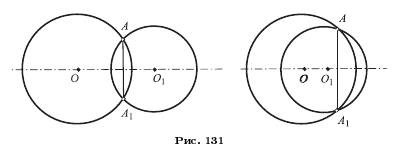
\includegraphics{mppics/ris-131}
\caption{}\label{1938/ris-131}
\end{figure}

Линия центров содержит в себе диаметры обеих окружностей и поэтому должна быть осью симметрии всей фигуры.
Поэтому общей точке $A$, лежащей вне линии центров, должна соответствовать симметричная общая точка $A_1$, расположенная по другую сторону от оси симметрии 
(на одном перпендикуляре к линии центров и на равном расстоянии от неё). 

\medskip

\smallskip
\so{Следствие}.
\emph{Общая хорда \emph{($AA_1$, рис.~\ref{1938/ris-131})} двух пересекающихся окружностей перпендикулярна к их линии центров и делится ею пополам.}

\paragraph{}\label{1938/119}
\so{Теорема}.
\textbf{\emph{Если две окружности имеют общую точку}} ($A$) \textbf{\emph{на линии их центров, то они касаются}} (рис.~\ref{1938/ris-132} и \ref{1938/ris-133}).

\begin{figure}[h!]
\begin{minipage}{.55\textwidth}
\centering
\includegraphics{mppics/ris-132}
\end{minipage}
\hfill
\begin{minipage}{.41\textwidth}
\centering
\includegraphics{mppics/ris-133}
\end{minipage}

\medskip

\begin{minipage}{.55\textwidth}
\centering
\caption{}\label{1938/ris-132}
\end{minipage}
\hfill
\begin{minipage}{.41\textwidth}
\centering
\caption{}\label{1938/ris-133}
\end{minipage}
\vskip-4mm
\end{figure}


Окружности не могут иметь другой общей точки вне линии центров, потому что в противном случае они имели бы ещё третью общую точку по другую сторону от линии центров и, следовательно, должны были бы слиться.
Они не могут иметь другой общей точки и на линии центров, так как, имея на этой линии две общие точки, они должны были бы иметь и общую хорду, соединяющую эти точки.
Но хорда, проходящая через центры, должна быть диаметром;
если же окружности имеют общий диаметр, то они сливаются в одну окружность.

\smallskip
\so{Замечание}.
Касание двух окружностей называется \rindex{внешнее касание}\textbf{внешним}, если окружности расположены одна вне другой (рис.~\ref{1938/ris-132}), и \rindex{внутреннее касание}\textbf{внутренним}, если одна из окружностей лежит внутри другой (рис.~\ref{1938/ris-133}).

\paragraph{}\label{1938/120}
\so{Теорема} (обратная предыдущей).
\textbf{\emph{Если две окружности касаются}} (в точке $A$, рис.~\ref{1938/ris-132} и \ref{1938/ris-133}), \textbf{\emph{то точка касания лежит на линии центров.}}

Точка $A$ не может лежать вне линии центров, потому что в противном случае окружности имели бы ещё другую общую точку, что противоречит условию теоремы (§~\ref{1938/118}).

\paragraph{}\label{1938/121}
\so{Следствие}.
\emph{Две касающиеся окружности имеют общую касательную в точке касания}, потому что, если проведём через точку касания прямую $MN$ (рис.~\ref{1938/ris-132} и \ref{1938/ris-133}), перпендикулярную к радиусу $OA$, то эта прямая будет также перпендикулярна и к радиусу $O_1A$.

\begin{figure}[h!]
\begin{minipage}{.54\textwidth}
\centering
\includegraphics{mppics/ris-134}
\end{minipage}
\hfill
\begin{minipage}{.42\textwidth}
\centering
\includegraphics{mppics/ris-135}
\end{minipage}

\medskip

\begin{minipage}{.54\textwidth}
\centering
\caption{}\label{1938/ris-134}
\end{minipage}
\hfill
\begin{minipage}{.42\textwidth}
\centering
\caption{}\label{1938/ris-135}
\end{minipage}
\vskip-4mm
\end{figure}

{\sloppy 
\paragraph{Различные случаи взаимного расположения двух окружностей.}\label{1938/122}
Обозначим радиусы двух окружностей буквами $R$ и $R_1$ и расстояние между их центрами буквой $d$.
Можно предположить, что $R_1\z\le R$.
Рассмотрим, какова зависимость между этими величинами в различных случаях взаимного расположения двух окружностей.
Этих случаев можно указать пять, а именно.

}

1) \so{Окружности лежат одна вне другой, не касаясь} (рис.~\ref{1938/ris-134});
в этом случае, очевидно, $d>R+R_1$.

2) \so{Окружности имеют внешнее касание} (рис. \ref{1938/ris-135});
тогда $d=R+R_1$, так как точка касания лежит на линии центров.

3) \so{Окружности пересекаются} (рис.~\ref{1938/ris-131});
тогда $d\z<R\z+R_1$ и в то же время $d>R-R_1$, потому что в $\triangle OAO_1$%
\footnote{На рис.~\ref{1938/ris-131} провести прямые $OA$ и $O_1A$.}
сторона $OO_1$, равная $d$, меньше суммы, но больше разности двух других сторон, равных радиусам $R$ и $R_1$.

4) \so{Окружности имеют внутреннее касание} (рис. \ref{1938/ris-133});
в этом случае $d=R-R_1$, потому что точка касания лежит на линии центров.

\begin{wrapfigure}{o}{47mm}
\centering
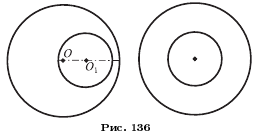
\includegraphics{mppics/ris-136}
\caption{}\label{1938/ris-136}
\end{wrapfigure}

5) \so{Одна окружность лежит внутри другой, не касаясь} (рис.~\ref{1938/ris-136});
тогда, очевидно, $d\z<R-R_1$, и в частном случае $d= 0$, когда центры обеих окружностей сливаются (такие окружности называются \rindex{концентрические окружности}\textbf{концентрическими}).


\smallskip
\mbox{\so{Замечание}.}
Учащимся предлагается проверить правильность обратных предложений, а именно:

1) \emph{Если $d>R+R_1$, то окружности расположены одна вне другой, не касаясь.}

2) \emph{Если $d=R+R_1$, то окружности касаются извне.}

3) \emph{Если $d<R+R_1$, и в то же время $d>R-R_1$, то окружности пересекаются.} 

4) \emph{Если $d=R-R_1$, то окружности касаются изнутри.}

5) \emph{Если $d<R-R_1$, то одна окружность лежит внутри другой, не касаясь.}

\smallskip
\so{Указание:} Все эти предложения легко доказываются от противного;
в доказательстве 3), следует воспользоваться допущением в §~\ref{1914/118}) % добавил указание

%???в 125--127(1996) содержит очень кривое обсуждение поворота — может и надо включить, но только полностью переписав
